\chapter{LightNVM 寫入流程之修改設計}
\indent
本論文為提升 Garbage Collection 的效率,以及降低 Garbage Collection 的次數,而提出此設計。透過實作新的演算法,將其與 LightNVM 既有的寫入流程結合,如此一來,LightNVM 在寫入時,會透過這個方法挑選寫入位置,以達成提升效率的目的。\\
\indent
修改大致可分為三部分,第一部分為初始化,讓原本 LightNVM 從準備一個 Line 變成準備四個 Line,一部分為 LightNVM 處理檔案系統的 Request,將資料存入 Ring Buffer;另一部分為 LightNVM 的 Write Thread 會被喚醒,檢查 Ring Buffer 並將 Entry 中紀錄的資料取出,寫到真正的SSD之中,本章節會解釋修改這兩部分的哪些環節。

\section{初始化時修改為準備四個 Line}\label{s3.1}
\indent
在初始化時,LightNVM 會先準備好一個 Line,後續有檔案系統傳遞給 LightNVM 寫入要求時,就會從這個 Line 開始寫入,滿了之後會繼續挑選下一個有空間的 Line 來使用,因此我們為了將資料分開寫入,要修改為在初始化時先準備好四個 Line,以便之後的寫入分群使用。

\begin{figure}[H]
    \centering
    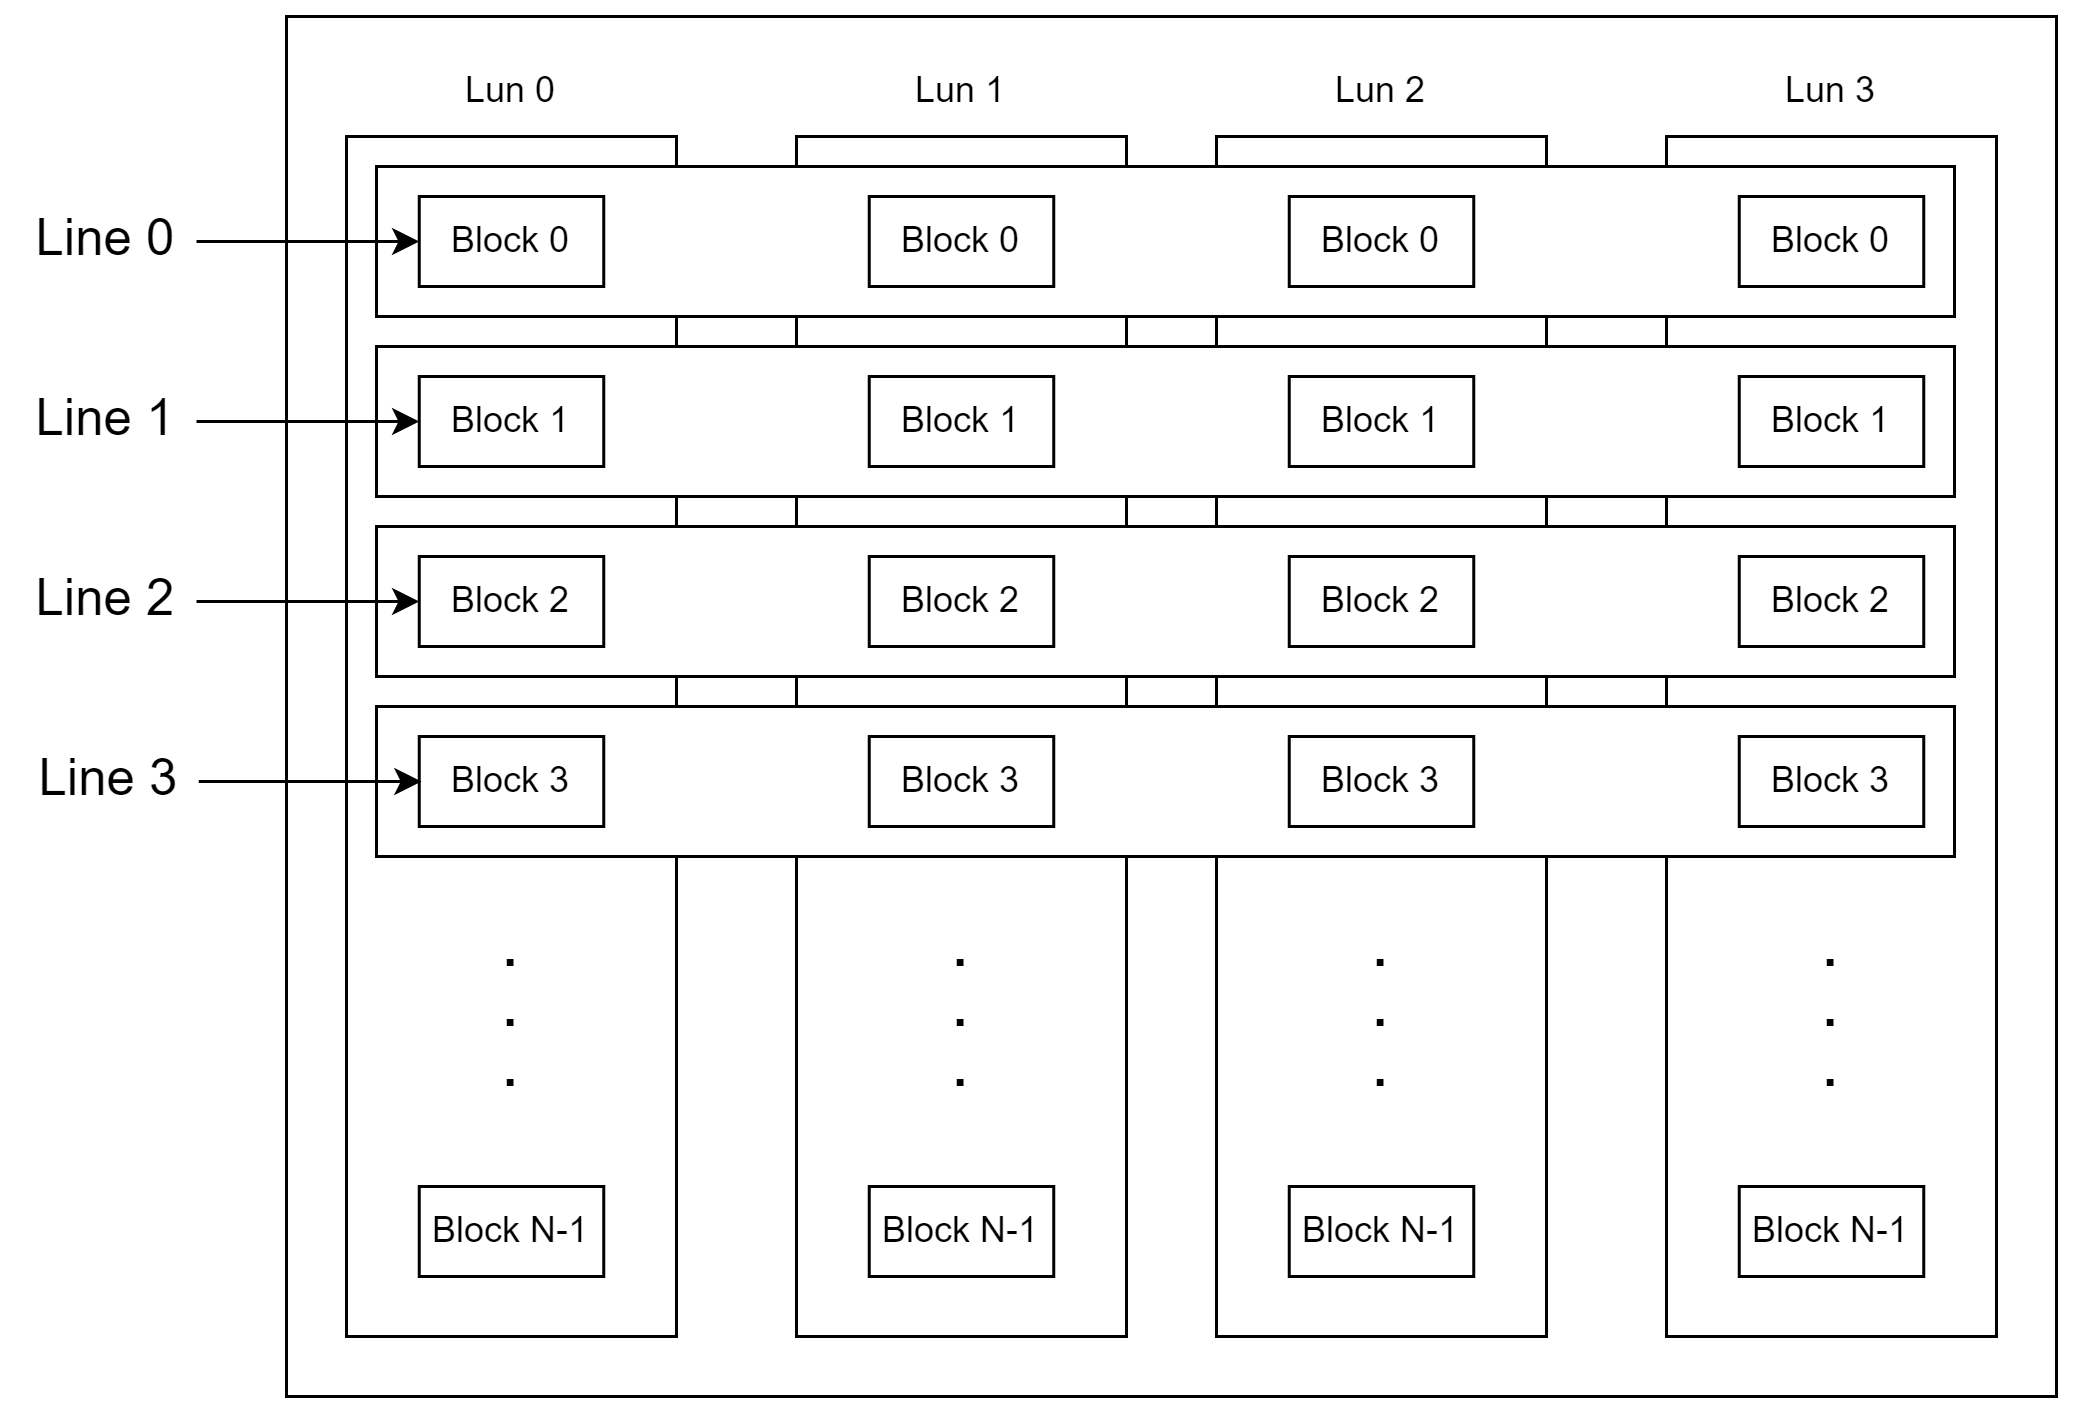
\includegraphics[width=1\textwidth]{picture/ch3/4Line.png}
    \caption{準備四個 Line}
    \label{f3.1}
\end{figure}

\section{處理檔案系統要求之流程}\label{s3.2}
\indent
檔案系統提出 Request 要求之後,LightNVM 會對 Request 拆解,儲存成 LightNVM 自己容易處理的形式,但是在拆解的同時,會損失一些資訊,所以首先我們要先在拆解 Request 之前把 Request 的大小先從 Request 的資料結構 bio (Block I/O) \cite{10.1145/2619092}擷取出來,用大小來判斷這個 Request 的資料屬於哪一個分群,並將資訊塞入 LightNVM 用來儲存 Request 的地方 - Ring Buffer 之中,最後再計算平均值,給下次 Request 傳進時使用。\cite{LightNVM}
\newpage

\subsection{以平均值劃分熱門資料及冷門資料}\label{s3.2.1}
\indent
首先為了劃分熱門以及冷門資料,我們將過去一萬筆 Request 大小的平均值當作基準,劃分四個等級,平均值的 0\% - 50\% 為最熱門的資料,平均值的 50\% - 100 \% 為第二熱門的資料,平均值的 100\% - 150\% 為第二冷門資料,平均值的 150\% 以上為最冷門的資料。並且由熱門到冷門,我們會分配到 Line 0 到 Line 3。
\begin{figure}[H]
    \centering
    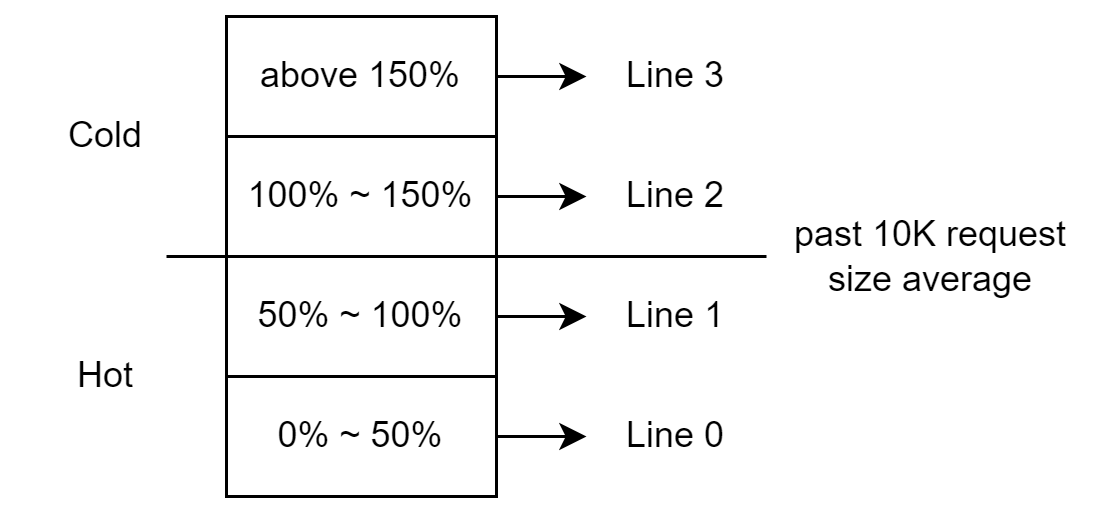
\includegraphics[width=0.7\textwidth]{picture/ch3/hot_cold.png}
    \caption{熱門資料與冷門資料}
    \label{f3.2}
\end{figure}

\subsection{擷取 Request 大小並判斷分群}\label{s3.2.2}
\indent
在得到 Request 大小時,我們需要從檔案系統傳給 LightNVM 的資料結構 bio 之中,找到 Request 大小的值;之後再以 Request 大小與平均值,判斷當下的 Request 屬於哪一類。
\begin{figure}[H]
    \centering
    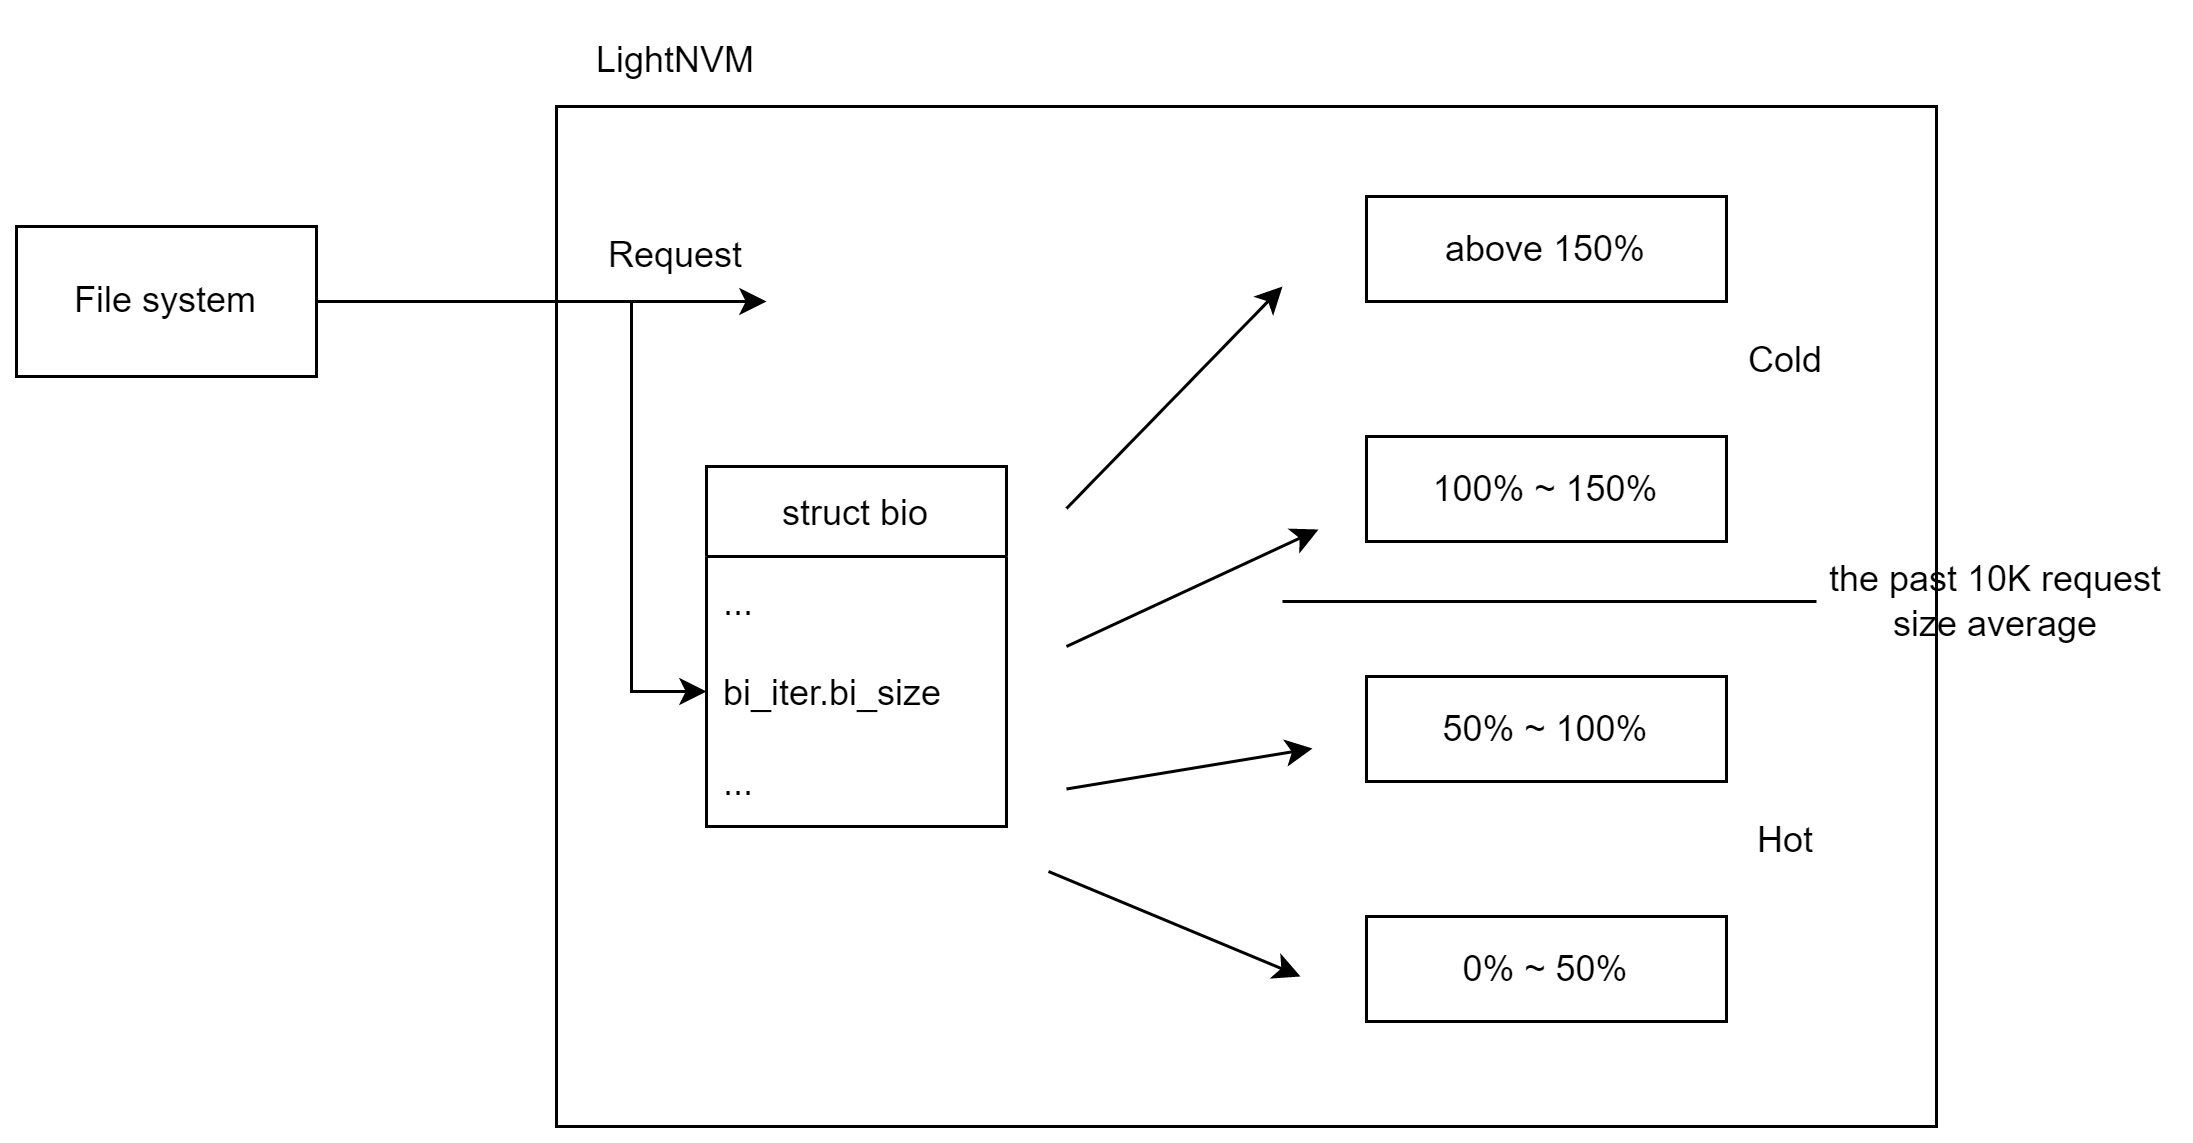
\includegraphics[width=1\textwidth]{picture/ch3/get_rq_size_hot_cold.png}
    \caption{判斷 Request 分群}
    \label{f3.3}
\end{figure}


\subsection{計算平均值}\label{s3.2.3}
\indent
在判斷完分群之後,我們需要拿剛剛得到的 Request 大小與平均值計算出新的平均值;由於我們需要前一萬筆 Request 大小的平均值,所以得到大小之後將其乘以 0.0001 倍再與我們加入 LightNVM 的平均值乘以 0.9999 倍之後相加,之後下一次檔案系統傳送 Request 進來時,就可以繼續用來判斷分群。
\begin{figure}[H]
    \centering
    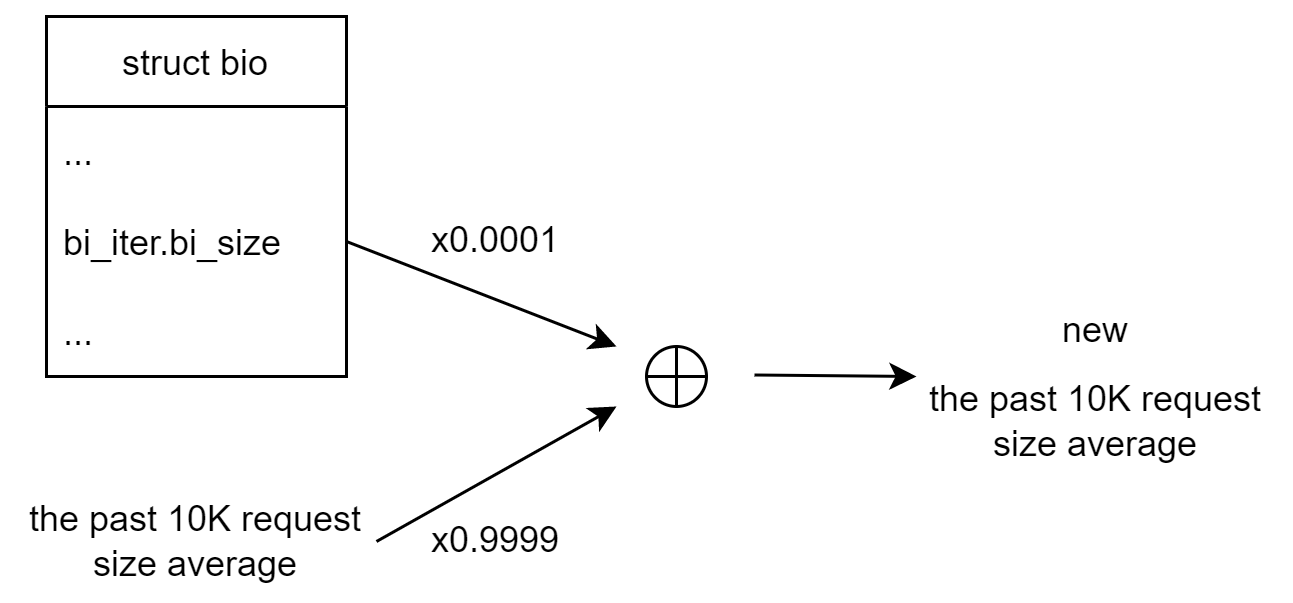
\includegraphics[width=0.8\textwidth]{picture/ch3/new_average.png}
    \caption{計算新平均值}
    \label{f3.4}
\end{figure}

\subsection{將 Request 所屬分群的資訊放入 Ring Buffer 中}\label{s3.2.4}
\indent
LightNVM 在接到檔案系統的 Request 之後,會將 Request 的資料拆解成數個 Page,每個 Page 都會記錄成 Ring Buffer 一個 Entry 之中,之後便會喚醒 LightNVM 背景的 write thread,從 Ring Buffer 存取剛剛放進去的 Entry,來得知寫入的資料位於 Host 記憶體,我們在這個 Entry 之中加入要存入哪個 Line,也就是冷熱分群的資訊,以便之後的 write thread 使用。

\begin{figure}[H]
    \centering
    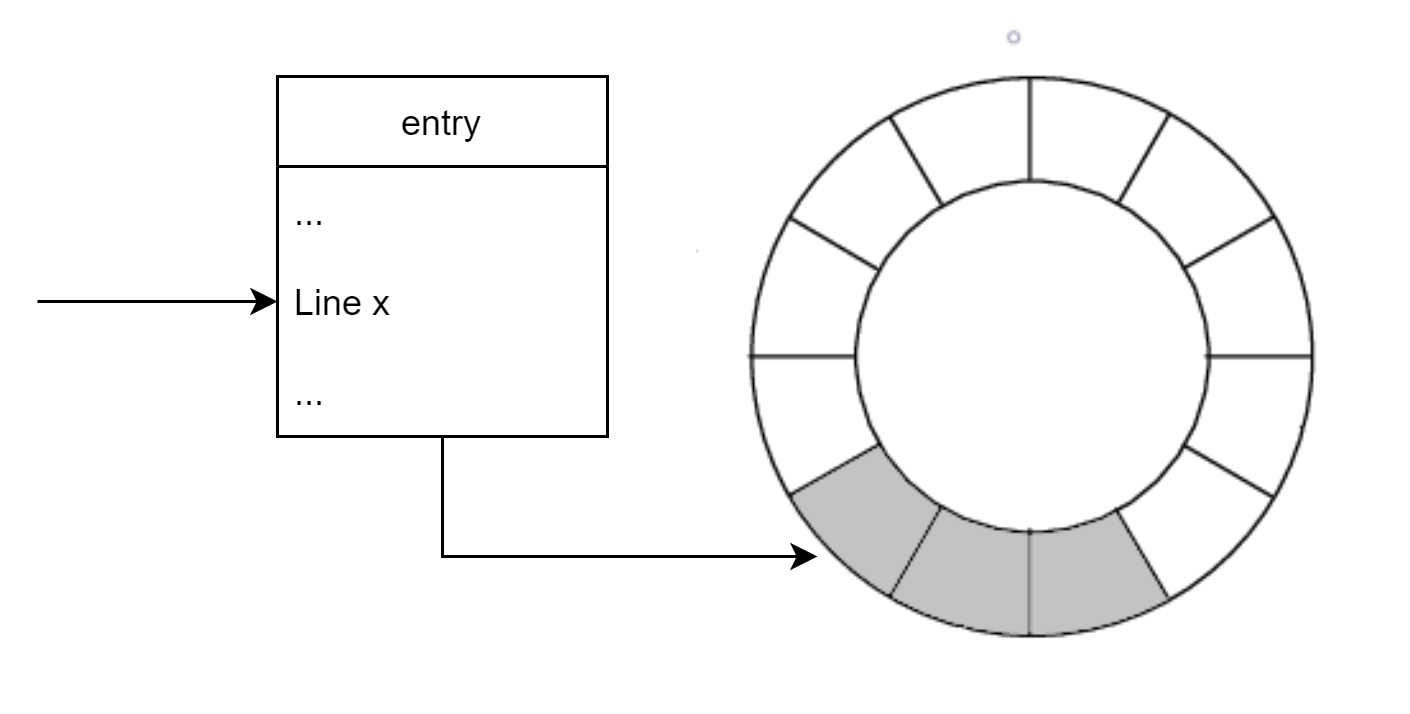
\includegraphics[width=0.7\textwidth]{picture/ch3/store_line_in_ring_buffer_entry.png}
    \caption{將分群資訊放入 Ring Buffer 的單位資料結構(Entry)}
    \label{f3.5}
\end{figure}

\section{實際寫入之過程}\label{s3.3}
\indent
LightNVM 的 Write Thread 被喚醒之後,會從剛剛紀錄到 Ring Buffer 之中的 Entry 得知要寫入的資料在哪裡,而我們也跟著得知剛剛我們放入的資訊,也就是每個 Entry 所屬的冷熱分群,接著我們將所有當次所提取的 Entry 的所屬冷熱分群總和之後取平均,得到的平均值就是我們最後寫入的 Line,最後我們將 Line 切換到我們的目標之後,LightNVM 就會根據我們所提供的 Line 來做 allocation,最終傳給 Open Channel SSD。

\subsection{從 Ring Buffer 中蒐集 Entry}\label{s3.3.1}
\indent
每次 LightNVM 從 Ring Buffer 之中抽取出的 Entry 數量不一定一樣,假設這次會取四個 Entry 的資料,分別所屬為 Line 3、2、1、2,那最後平均值是 2。

\begin{figure}[H]
    \centering
    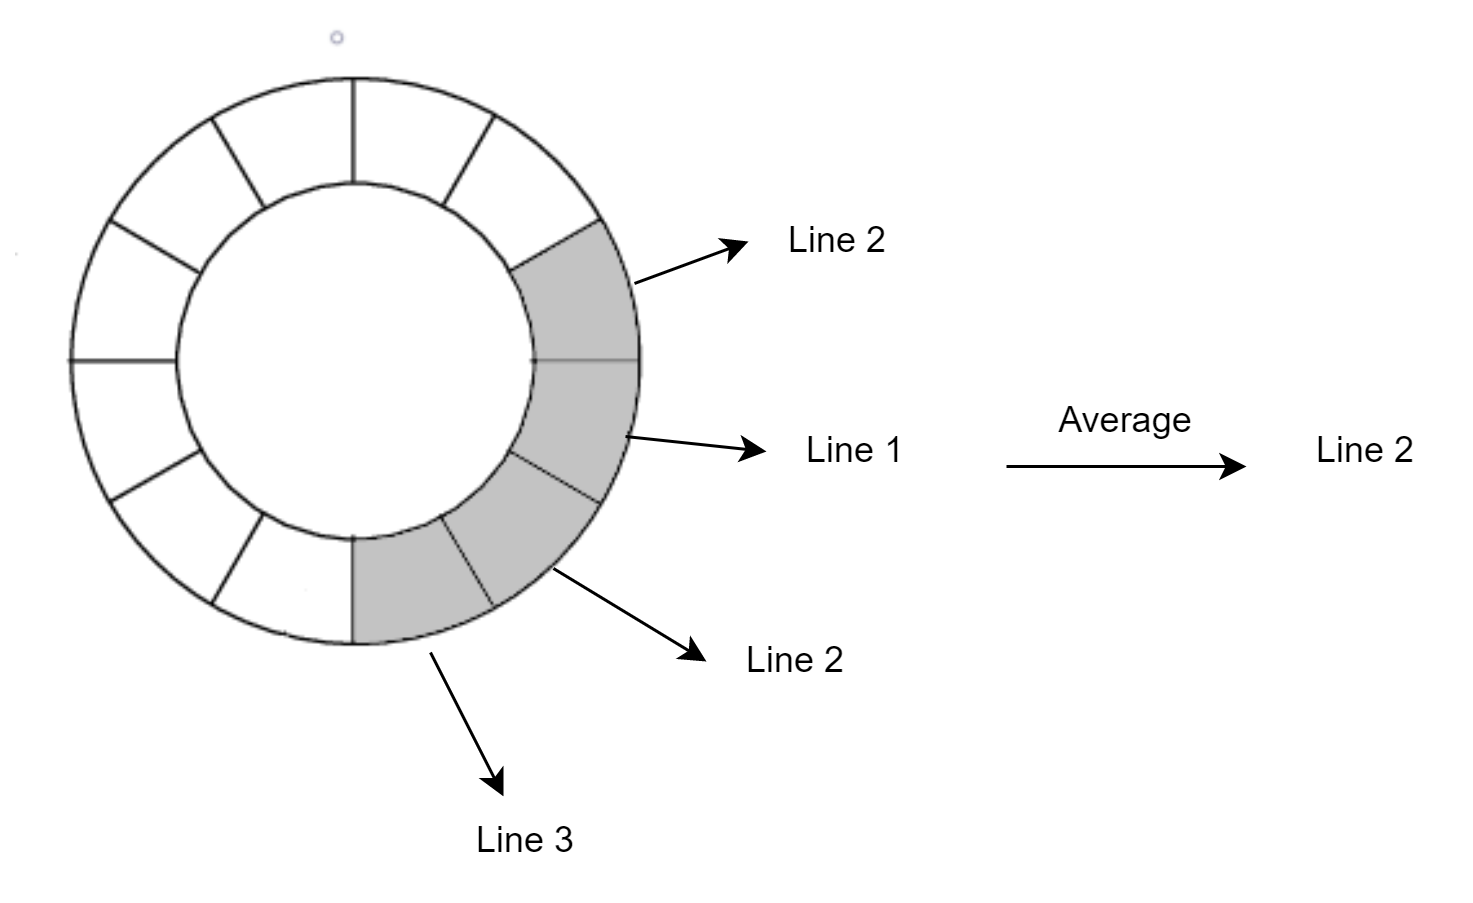
\includegraphics[width=0.7\textwidth]{picture/ch3/get_entry_from_ring_buffer.png}
    \caption{從數個 Entry 取出 Line 之後平均}
    \label{f3.6}
\end{figure}

\subsection{切換 Line 之後傳送給 Open Channel SSD}\label{s3.3.2}
\indent
按照剛剛計算的平均值切換 Line 之後,LightNVM 會根據我們指定的 Line 做 Allocation,最後將資料以及位置往下傳給 Open Channel SSD(圖例延續 \ref{s3.3.1})。
\begin{figure}[H]
    \centering
    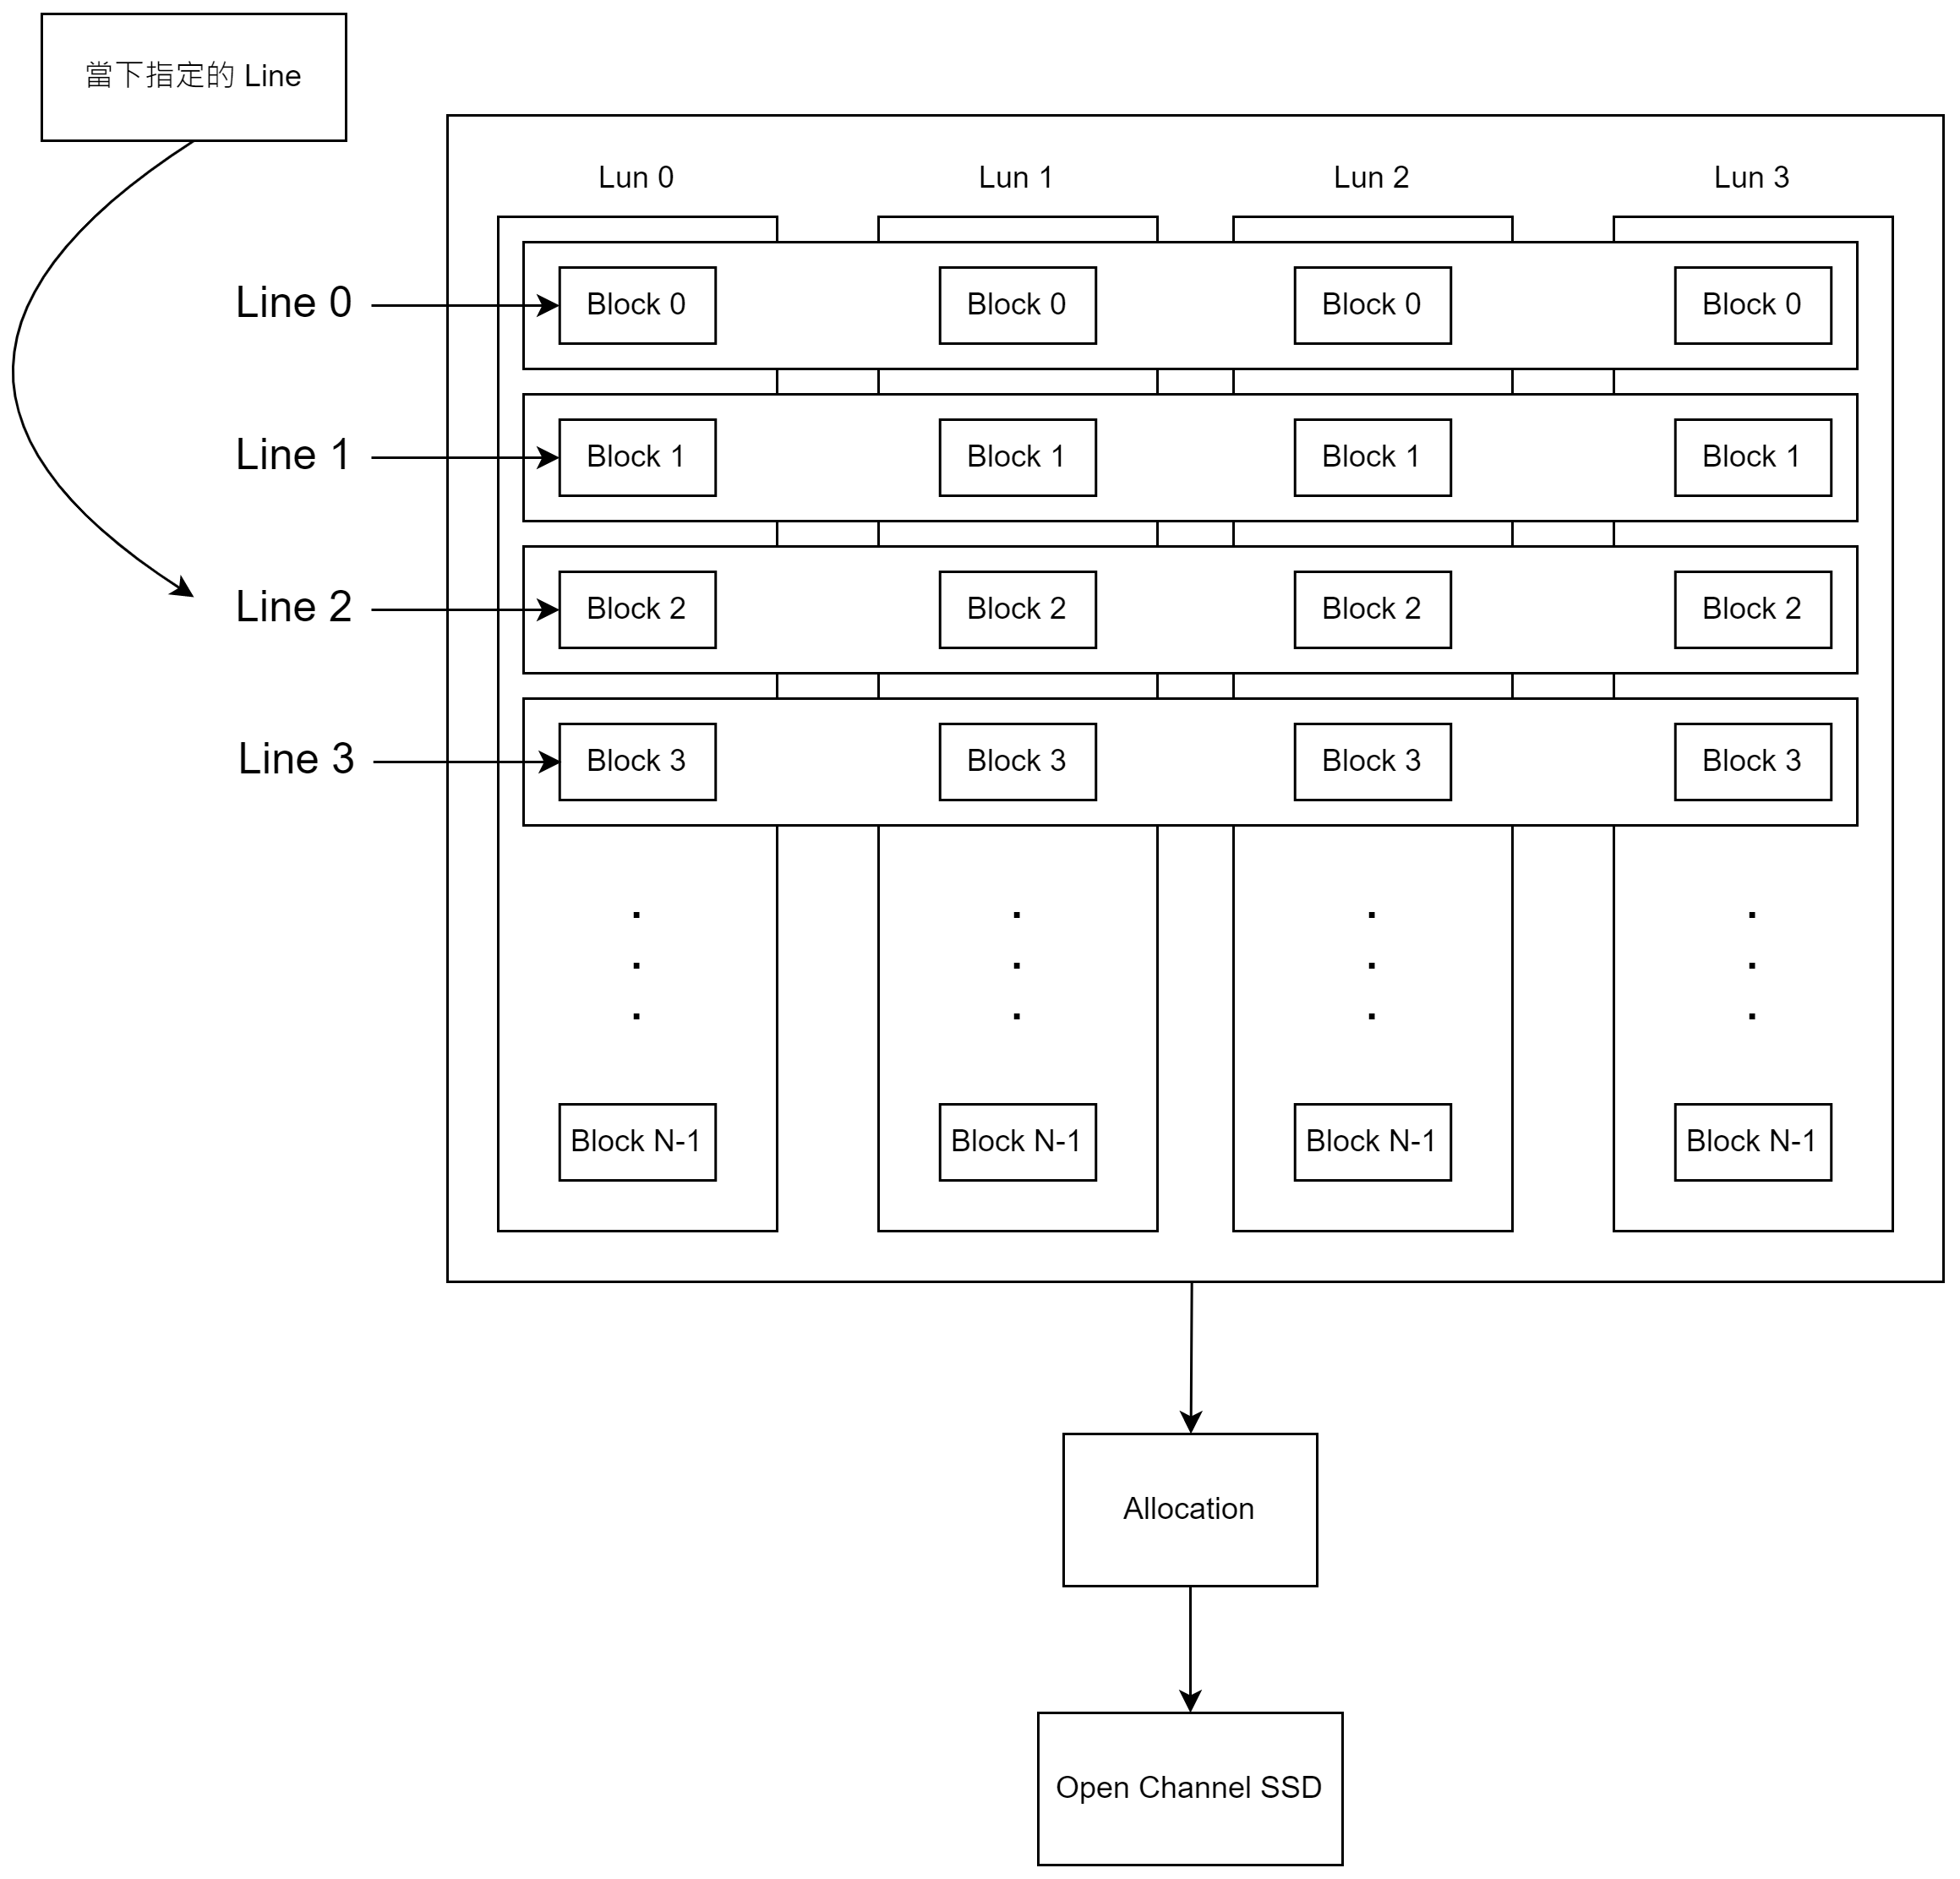
\includegraphics[width=1\textwidth]{picture/ch3/switch_line_to_opssd.drawio.png}
    \caption{切換 Line 之後 Allocation,最後傳給 Open Channel SSD}
    \label{f3.7}
\end{figure}
%\subsection{建立開發外掛程式之環境}
%\indent
%Plug-in Development Environment(PDE)\cite{PDE}是Eclipse中提供開發人員進行外掛程式開發的工具,其中提供了多種協助開發的功能,例如:創立專案、除錯、測試、建置專案、部屬等等。本論文將在PDE中引入既有外掛程式之專案,進行新重構功能之擴充。

%\subsection{利用Eclipse中延伸點與應用程式介面進行擴充}
%\indent
%\ref{s2.4}節中提及了Eclipse的擴充機制,而Eclipse中含有十分豐富的延伸點與各種應用程式介面,透過不同的延伸點與應用程式介面的結合,外掛程式可以更多元地使用Eclipse上的各種功能,例如:監聽使用者操作進而做出後續反應、取得工作區檔案中的各項資訊提供外掛程式使用等等。本論文透過此擴充機制能夠更加簡化使用者重構之動作,且更方便地新增重構功能。

%\subsection{增加command元素}\label{s3.4.3}
%\indent
%在Eclipse中command是一個行為的描述,但與實際行為操作並無相關,其行為操作是由handler所定義,而一個command可以擁有多個handler,但在一個時間點上只會將行為託付給一個handler。Eclipse提供了commands的延伸點,開發人員能夠藉此新增command以及定義其種類。本論文將為已有三個command的commands延伸點進行擴充,新增兩個command,分別為抽取重複步驟成為新關鍵字、移動關鍵字宣告,後續將新增handler為其定義實際行為。圖\ref{f3.9}為現有commands之延伸點。
%
%\begin{figure}[H]
%    \centering
%    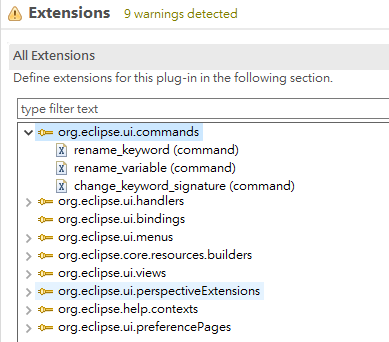
\includegraphics[width=0.8\textwidth]{picture/command_extension.PNG}
%    \caption{外掛程式現有之commands延伸點3}
%    \label{f3.9}
%\end{figure}
%
%\subsection{透過handler定義新command的行為}
%\indent
%Eclipse提供了handlers的延伸點,讓開發人員能夠進行handler與command的連接,並且設定handler在不同條件下為啟用、禁用或非活動的狀態,如果handler處於禁用狀態,儘管收到了command的委託,也不會執行,而處於非活動的狀態時,command將不會被委託至此handler,因此在啟用狀態下,command將會委託此handler執行行為。本論文將為已有三個handler的handlers延伸點新增兩個handler,並將其與\ref{s3.4.3}節中的command進行連接,完成相對應的重構行為。圖\ref{f3.10}為現有handlers之延伸點。
%
%\begin{figure}[H]
%    \centering
%    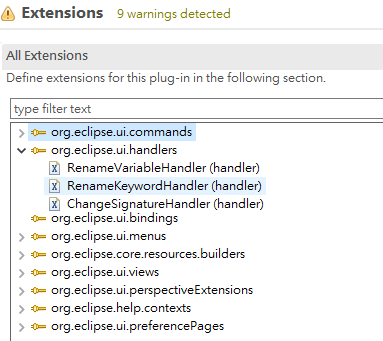
\includegraphics[width=0.8\textwidth]{picture/handler_extension.PNG}
%    \caption{外掛程式現有之handlers延伸點}
%    \label{f3.10}
%\end{figure}
%
%\subsection{將新command與選單介面結合}
%\indent
%Eclipse提供了menus的延伸點,讓開發人員能夠將客製化的選單新增至Eclipse框架上,提供使用者能夠操作其所需之功能,其中提供了以下幾種選單種類:
%
%\begin{itemize}
%
%\item\textbf{主選單(Main menu)}
%
%\item\textbf{主工具列(Main toolbars)}
%
%\item\textbf{修剪選單(Trim)}
%
%\item\textbf{視圖選單/工具列(View menus/Toolbars)}
%
%\end{itemize}
%
%\indent
%此外選單介面可與不同元件結合,例如:control、command、menu等等,讓客製化選單能夠更加多元。本論文將於現有menus延伸點的客製化選單中,結合\ref{s3.4.3}節中所新增之command,讓使用者能夠依照其需求選擇選單中的功能,並將command委託至handler執行。圖\ref{f3.11}為現有menus之延伸點。
%
%\begin{figure}[H]
%    \centering
%    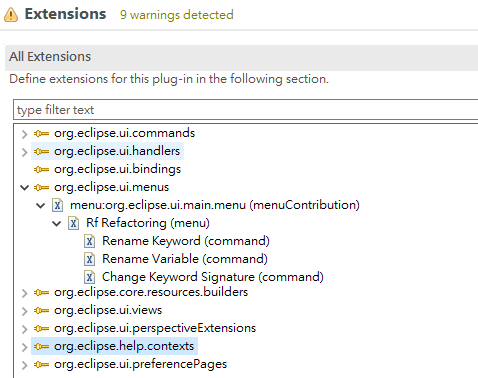
\includegraphics[width=0.8\textwidth]{picture/menu_extension.PNG}
%    \caption{外掛程式現有之menus延伸點}
%    \label{f3.11}
%\end{figure}

%\subsection{透過視圖及視窗協助重構功能執行}
%\indent
%Eclipse提供了views延伸點,開發人員可藉此新增客製化的視圖(View),而視圖為工作區內的可視化元件,其可被用來顯示command執行結果資訊或新增額外的使用者元件等等,圖\ref{f3.12}為現有外掛程式的客製化視圖,其提供使用者選擇所要重新命名的參考。本論文將於現有views延伸點新增兩個不同的客製化視圖,分別提供使用者選擇重複步驟或目標檔案,以此協助重構功能之執行。
%
%\begin{figure}[H]
%    \centering
%    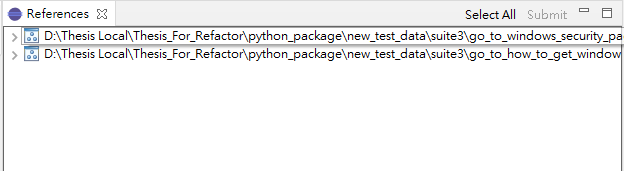
\includegraphics[width=1.0\textwidth]{picture/choose_keyword_view.PNG}
%    \caption{現有外掛程式的客製化視圖}
%    \label{f3.12}
%\end{figure}
%
%\indent
%視窗(Dialog)是SWT(Standard Widget Toolkit)\cite{SWT}中所提供的視窗元件,其可透過開發人員自行設計介面,以達到所需之功能,圖\ref{f3.13}為現有外掛程式的客製化視窗,其提供使用者輸入重新命名的關鍵字名稱。本論文將新增兩個視窗介面,提供使用者創建新關鍵字及用新關鍵字取代重複步驟之功能使用,協助整體重構功能之執行。
%
%\begin{figure}[H]
%    \centering
%    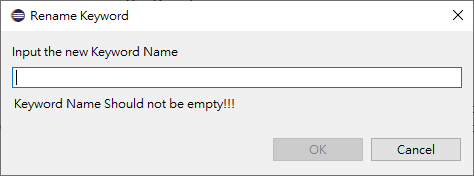
\includegraphics[width=0.7\textwidth]{picture/Rename_keyword_dialog.PNG}
%    \caption{現有外掛程式的客製化視窗}
%    \label{f3.13}
%\end{figure}